\sectionpic{Vectors}{../figures/presentation_chapters/vectors.pdf}

\begin{frame}
  \frametitle{Basics of Vectors}
  There are 3 distinct approaches to describe what a vector is:
  \begin{itemize}
  \item The physicist's approach (geometric)
  \item The computer scientist's approach (algebraic)
  \item The mathematician's approach (abstract)
  \end{itemize}
\end{frame}

\begin{frame}
  \frametitle{Geometric Vectors}
  \begin{presentation_definition}
  A vector is an object with a length and a direction.
  \end{presentation_definition}

  \begin{figure}[H]
  \centering
  \begin{tikzpicture}[scale=0.75, align=center]
  \Large
  \draw[vector, col1] (0,0) -- (2,3);
  \draw[vector, col2] (-1,0) -- (-2,2);
  \draw[vector, col3] (0,-1) -- (-3,-1);
  \draw[vector, col4] (2,0) -- (1,-3);
  \draw[vector, col5] (-4,2) -- (-4,-2);
  \draw[vector, black] (-7,1) -- (-6,0);
  \end{tikzpicture}
  \end{figure}
\end{frame}

\begin{frame}
  \frametitle{Vector Notation}
  Vectors are denoted as latin letters with an arrow above them:
  \begin{equation*}
  \vec{u},\quad\vec{v},\quad\vec{x},\quad\vec{a},\quad\cdots
  \end{equation*}

  In maths and physics the following notations are mostly used:
  \begin{align*}
  \bm{u},\quad\bm{v},\quad\bm{x},\quad\bm{a},\quad\cdots\\
  \underline{\bm{u}},\quad\underline{\bm{v}},\quad\underline{\bm{x}},\quad\underline{\bm{a}},\quad\cdots\\
  \end{align*}
\end{frame}

\begin{frame}
  \frametitle{Geometric Vectors}
  We consider all vectors starting at the same point, called the \emph{origin}.

  \begin{figure}[H]
  \centering
  \begin{tikzpicture}[scale=0.75, align=center]
  \draw[vector, col1] (0,0) -- (2,3);
  \draw[vector, col2] (0,0) -- (-1,2);
  \draw[vector, col3] (0,0) -- (-3,0);
  \draw[vector, col4] (0,0) -- (-1,-3);
  \draw[vector, col5] (0,0) -- (0,-4);
  \draw[vector, black] (0,0) -- (1,-1);
  \filldraw[black] (0,0) circle (0.05);
  \end{tikzpicture}
  \end{figure}
\end{frame}

\begin{frame}
  \frametitle{Scaling Vectors}
  We can multiply a vector by a real number, which we refer to as a \emph{scalar}. This scales only the length of the vector while keeping its direction on the same line as before:
  \begin{figure}[H]
  \centering
  \begin{tikzpicture}[scale=0.75, align=center, every node/.style={midway, above}]
  \Large
  \draw [vector, col1] (0,0) -- ++(1.5,1) node {$\vec{v}$};
  \draw [vector, col2] (2,0) -- ++(3,2) node {$2\vec{v}$};
  \draw [vector, col4] (4,0) -- ++(4.5,3) node [xshift=-1mm] {$3\vec{v}$};
  \draw [vector, <-, thick, col6] (6,0) -- ++(1.5,1) node [xshift=-2mm] {$-1\vec{v}$};
  \draw [vector, <-, thick, black] (8,0) -- ++(3,2) node [xshift=-2mm] {$-2\vec{v}$};
  \end{tikzpicture}
  \end{figure}
\end{frame}

\begin{frame}
  \frametitle{Vector Addition}
  Adding two vectors is done by placing the origin of one vector at the head of the other vector. The addition results in a vector starting at the first vector’s origin and ending at the second vector’s head:

  \vspace{1cm}
  \begin{figure}[H]
  \centering
  \begin{tikzpicture}
  \Large
  \coordinate (o) at (0,0);
  \coordinate (u) at (-2,1);
  \coordinate (v) at (3,2);
  \coordinate (w) at ($(u)+(v)$);
  \onslide<1->{
  \draw[vector, col1] (o) -- ++(u) node[above left] {$\vec{u}$};
  }
  \onslide<1,4>{
  \draw[vector, col2] (o) -- ++(v) node[above left] {$\vec{v}$};
  }
  \onslide<2-3>{
  \draw[vector, col2] (u) -- ++(v) node[above left] {$\vec{v}$};
  }
  \onslide<3->{
  \draw[vector, col4] (o) -- ++($(u)+(v)$) node[below right] {$\vec{w}$};
  }
  \filldraw[black] (o) circle (0.05);
  \end{tikzpicture}
  \end{figure}
\end{frame}

\begin{frame}
  \frametitle{Vector Addition}
  Notice that adding vectors is a commutative operation, i.e.
  \begin{equation*}
  \rcolor{col1}{\vec{u}}+\rcolor{col2}{\vec{v}} = \rcolor{col2}{\vec{v}}+\rcolor{col1}{\vec{u}}
  \end{equation*}

  \begin{figure}[H]
  \centering
  \begin{tikzpicture}[every node/.style={midway, above}]
  \draw[vector, col1] (o) -- ++(u) node {$\vec{u}$};
  \draw[vector, col2] (o) -- ++(v) node {$\vec{v}$};
  \draw[vector, col1] (v) -- ++(u) node {$\vec{u}$};
  \draw[vector, col2] (u) -- ++(v) node {$\vec{v}$};
  \draw[vector, col4] (o) -- ++($(u)+(v)$) node [left] {$\vec{w}$};
  \filldraw[black] (o) circle (0.05);
  \end{tikzpicture}
  \end{figure}

  \onslide<2>{
  This is refered to as the \emph{parallelogram law of vector addition}.
  }
\end{frame}

\begin{frame}
  \frametitle{The Zero Vector}
  And important vector is the \emph{zero vector}, which has a length of $0$ and no direction. It is notated as $\vec{0}$, and is neutral to addition, i.e. for any vector $\vec{v}$:
  \begin{equation*}
  \vec{v}+\vec{0} = \vec{0}+\vec{v} = \vec{v}.
  \end{equation*}

  \onslide<2->{
  Similarily, any addition of a vector with its opposite vector results in the zero vector:
  \begin{equation*}
  \vec{v} + \left(-\vec{v}\right) = -\vec{v} + \vec{v} = \vec{0}.
  \end{equation*}
  }
\end{frame}

\begin{frame}
  \frametitle{Algebraic Vectors}
  \begin{onlyenv}<1>
  Placing a vector in a cartesian coordinate system:
  \end{onlyenv}
  \begin{onlyenv}<2>
  Then, drawing a perpendicular from $\vec{v}$ to the $x$-axis:
  \end{onlyenv}
  \begin{onlyenv}<3>
  And similarily for the $y$-axis:
  \end{onlyenv}
  \begin{onlyenv}<4>
  We call $u_{x}$ and $u_{y}$ the \emph{components} of $\vec{u}$.
  \end{onlyenv}
  \begin{figure}[H]
  \centering
  \begin{tikzpicture}
  \Large

  % Coordinate
  \coordinate (u) at (4,3);

  %\onslide<4->{
  %  % Angle
  %  \filldraw[-, thick, fill=col3!30] (0,0) -- (1.5,0) arc (0:36.9:1.5) -- (0,0);
  %  \node at (1,0.34) {$\theta$};
  %}

  \onslide<1->{
  % Vector
  \draw[vector, ultra thick, col1] (o) -- ++(u) node [above right] {$\vec{u}$};

  % Axes
  \draw[vector, <->] (-1,0) -- (5,0) node [right] {$x$};
  \draw[vector, <->] (0,-1) -- (0,5) node [above] {$y$};
  }

  % Perpendiculars
  \coordinate (dx) at (0.25,0);
  \coordinate (dy) at (0,0.25);
  \coordinate (-dx) at (-0.25,0);
  \coordinate (-dy) at (0,-0.25);
  \onslide<2->{
  \draw[perp] (u) -- (u|-o) node [below] {$u_{x}$};
  \draw[-, thick] ($(u|-o)+(dy)$) -- ++(-dx) -- ++(-dy);
  \filldraw (u|-o) circle (0.05);
  }
  \onslide<3->{
  \draw[perp] (u) -- (u-|o) node [left] {$u_{y}$};
  \draw[-, thick] ($(u-|o)+(dx)$) -- ++(-dy) -- ++(-dx);
  \filldraw (u-|o) circle (0.05);
  }

  % Components
  \onslide<4->{
  \draw [col2, thick, decorate, decoration={brace, amplitude=3pt, raise=3pt, mirror}]
  (o) -- ++(u|-o) node[midway, below , yshift=-5pt]{$x$-component};
  \draw [col3, thick, decorate, decoration={brace, amplitude=3pt, raise=3pt}]
  (o) -- ++(u-|o) node[rotate=90, left, yshift=15pt]{$y$-component};
  }
  \end{tikzpicture}
  \end{figure}
\end{frame}

\begin{frame}
  \frametitle{Column Vectors}
  We then notate the vector $\vec{u}$ as a \emph{column vector} with components $u_{x},u_{y}$:
  \begin{equation*}
  \vec{u} = \colvec{2}{u_{x}}{u_{y}}.
  \end{equation*}

  Since $\vec{u}$ has two real components, it is a member of $\Rs{2}$.
\end{frame}

\begin{frame}
  \frametitle{Higher-dimensional Vectors}
  This scheme can be extended to 3-dimensional vectors:
  \begin{figure}[H]
  \centering
  \begin{tikzpicture}[scale=0.75, every path/.style={->, >=stealth, very thick},
  scale=1.5]
  \Large

  \pgfmathsetmacro{\vx}{3};
  \pgfmathsetmacro{\vy}{2};
  \pgfmathsetmacro{\vz}{2};
  \coordinate (v) at (\vx,\vy,\vz);
  \coordinate (vxz) at (\vx, 0, \vz);
  \coordinate (dx) at (0.25,0,0);
  \coordinate (dy) at (0,0.25,0);
  \coordinate (dz) at (0,0,0.25);
  \coordinate (-dx) at (-0.25,0,0);
  \coordinate (-dy) at (0,-0.25,0);
  \coordinate (-dz) at (0,0,-0.25);
  \coordinate (dxz) at (0.21,0,0.14);

  \pgfmathsetmacro{\alen}{4};
  \draw[vector] (o) to (\alen,0,0) node [right] {$x$};
  \draw[vector] (o) to (0,\alen,0) node [above] {$y$};
  \draw[vector] (o) to (0,0,\alen) node [below left] {$z$};

  \draw[perp, col2] (vxz) -- (\vx,0,0) node [above] {$v_{x}$};
  \draw[perp, black!20] (v) -- (vxz);
  \draw[perp, col3] (v) -- (0,\vy,0) node [left] {$v_{y}$};
  \draw[perp, black!20] (vxz) -- (o);
  \draw[perp, col4] (vxz) -- (0,0,\vz) node [left] {$v_{z}$};
  \draw[vector, col1] (o) to (v) node [above right] {$\vec{v}$};

  \draw[-, thick] ($(\vx,0,0)+(-dx)$) -- ++(dz) -- ++(dx);
  \draw[-, thick] ($(0,\vy,0)+(-dy)$) -- ++(dxz) -- ++(dy);
  \draw[-, thick] ($(0,0,\vz)+(-dz)$) -- ++(dx) -- ++(dz);
  \end{tikzpicture}
  \end{figure}
\end{frame}

\begin{frame}
  \frametitle{Higher-dimensional Vectors}
  \onslide<1->{
  A column vector in $\Rs{3}$ looks as following:
  \begin{equation*}
  \vec{v} = \colvec{3}{v_{x}}{v_{y}}{v_{z}},
  \end{equation*}
  }
  \onslide<2->{
  and in $\Rs{4}$:
  \begin{equation*}
  \vec{a} = \colvec{4}{v_{x}}{v_{y}}{v_{z}}{v_{w}}.
  \end{equation*}
  }
\end{frame}

\begin{frame}
  \frametitle{Higher-dimensional Vectors}
  A general column vector in $\Rs{n}$ looks as following:
  \begin{equation*}
  \vec{v} = \colvec{4}{v_{1}\tikzmark{v1}}{v_{2}}{\vdots}{v_{n}\tikzmark{vn}}
  \end{equation*}
  \begin{tikzpicture}[overlay, remember picture]
  \node [above right=of v1, xshift=-8mm, yshift=-5mm] (v1b) {};
  \node [below right=of vn, xshift=-8mm, yshift= 8mm] (vnb) {};
  \draw [col1, thick, decorate, decoration={brace, amplitude=3pt, raise=3pt}]
  (v1b) -- (vnb) node[midway, right, xshift=10pt]{$n$ components};
  \end{tikzpicture}
\end{frame}

\begin{frame}
  \frametitle{The Zero Vector}
  As a column vector, the zero vector in $\Rs{2}$ is
  \begin{equation*}
  \vec{0} = \colvec{2}{0}{0}.
  \end{equation*}

  \onslide<2->{
  In $\Rs{3}$ it is
  \begin{equation*}
  \vec{0} = \colvec{3}{0}{0}{0}.
  \end{equation*}
  }

  \onslide<3->{
  And generally, in $\Rs{n}$, it is
  \begin{equation*}
  \vec{0} = \colvec{4}{0\tikzmark{01}}{0}{\vdots}{0\tikzmark{0n}}
  \end{equation*}
  \begin{tikzpicture}[overlay, remember picture]
  \node [above right=of 01, xshift=-8mm, yshift=-5mm] (01b) {};
  \node [below right=of 0n, xshift=-8mm, yshift= 8mm] (0nb) {};
  \draw [col1, thick, decorate, decoration={brace, amplitude=3pt, raise=3pt}]
  (01b) -- (0nb) node[midway, right, xshift=10pt]{$n$ components};
  \end{tikzpicture}
  }
\end{frame}

\begin{frame}
  \frametitle{Length and Angle of a Vector}
  \begin{onlyenv}<1>
  Using the Pythagorean theorem to calculate the length (norm) of a vector in $\Rs{2}$:
  \begin{equation*}
  \norm{\rcolor{col1}{\vec{u}}} = \sqrt{\rcolor{col2}{u}^{2}_{\rcolor{col2}{{x}}} + \rcolor{col3}{u}^{2}_{\rcolor{col3}{{y}}}}.
  \end{equation*}
  \end{onlyenv}
  \begin{onlyenv}<2>
  The angle $\rcolor{col4}{\theta}$ is then:
  \begin{equation*}
  \tan(\rcolor{col4}{\theta}) = \frac{\rcolor{col3}{u_{y}}}{\rcolor{col2}{u_{x}}}.
  \end{equation*}
  \end{onlyenv}

  \begin{figure}[H]
  \centering
  \begin{tikzpicture}[scale=0.75]
  \Large

  % Coordinate
  \coordinate (u) at (4,3);
  \coordinate (oo) at (4,0);
  \coordinate (uo) at ($(o)+(u)$);

  % Angle
  \onslide<2->{
  %\filldraw[-, thick, draw=col4, fill=col4!20] (0,0) -- (1.5,0) arc (0:36.9:1.5) -- (0,0);
  %\node[text=col4] at (1,0.34) {$\theta$};
  \filldraw[col4!20, draw=col4, thick] let
  \p1=(u), \p2=(oo), \n1={atan2(\y1,\x1)}, \n2={atan2(\y2,\x2)}
  in (o) -- ($(o)!1.5cm!(oo)$) arc[start angle=\n2, end angle=\n1, radius=1.5cm]
  node [text=col4] at ($(o)!1cm!(uo) + (1.5mm,-2.5mm)$) {$\theta$};
  }

  % Vector
  \draw[vector, ultra thick, col1] (o) -- node [midway, above] {$\vec{u}$} ++(u);

  % Axes
  \xaxis{-1}{5}
  \yaxis{-1}{5}

  % Perpendiculars
  \coordinate (dx) at (0.25,0);
  \coordinate (dy) at (0,0.25);
  \coordinate (-dx) at (-0.25,0);
  \coordinate (-dy) at (0,-0.25);
  \draw[perp] (u) -- (u|-o);
  \draw[-, thick] ($(u|-o)+(dy)$) -- ++(-dx) -- ++(-dy);

  % Components
  \draw [col3, thick, decorate, decoration={brace, amplitude=3pt, raise=3pt}]
  (u) -- (u|-o) node[midway, right, xshift=5pt]{$u_{y}$};
  \draw [col2, thick, decorate, decoration={brace, amplitude=3pt, raise=3pt, mirror}]
  (o) -- (u|-o) node[midway, below, yshift=-5pt]{$u_{x}$};

  \end{tikzpicture}
  \end{figure}
\end{frame}

\begin{frame}
  \frametitle{Length of a Vector}
  Similarily, the length of a column vector in $\Rs{3}$, $\vec{v}=\colvec{3}{v_{x}}{v_{y}}{v_{z}}$ is
  \begin{equation*}
  \norm{\vec{v}} = \sqrt{v_{x}^{2} + v_{y}^{2} + v_{z}^{2}}.
  \end{equation*}
\end{frame}

\begin{frame}
  \frametitle{Length of a Vector}
  \begin{presentation_challenge}
  Show that the above given formula is true, i.e. show that for a box of sides $\rcolor{col2}{a},\rcolor{col5!75}{b},\rcolor{col4}{c}$, the length of the line from A to B (see figure) is indeed $\sqrt{\rcolor{col2}{a}^{2} + \rcolor{col5!75}{b}^{2} + \rcolor{col4}{c}^{2}}$.
  \begin{figure}[H]
  \centering
  \begin{tikzpicture}[every path/.style={very thick}, node distance=1mm]
  \pgfmathsetmacro{\xside}{4};
  \pgfmathsetmacro{\yside}{2};
  \pgfmathsetmacro{\zside}{3};

  \coordinate (1) at (0,0,0);
  \coordinate (2) at (\xside,0,0);
  \coordinate (3) at (0,\yside,0);
  \coordinate (4) at (\xside,\yside,0);
  \coordinate (5) at (0,0,\zside);
  \coordinate (6) at (\xside,0,\zside);
  \coordinate (7) at (0,\yside,\zside);
  \coordinate (8) at (\xside,\yside,\zside);

  \draw (1) -- (2);
  \draw (1) -- (3);
  \draw (1) -- (5);
  \draw[densely dotted, red] (5) -- (4);
  \draw (5) -- (7);
  \draw (6) -- (8);
  \draw (2) -- (4);
  \draw (2) -- (6);
  \draw (3) -- (4);
  \draw (3) -- (7);
  \draw (4) -- (8);
  \draw (5) -- (6);
  \draw (7) -- (8);

  \node[left=of 5] {$A$};
  \node[above=of 4] {$B$};

  \draw [col2, thick, decorate, decoration={brace, amplitude=3pt, raise=3pt, mirror}]
  (5) -- (6) node[midway, below, yshift=-5pt]{$a$};
  \draw [col5!75, thick, decorate, decoration={brace, amplitude=3pt, raise=3pt, mirror}]
  (6) -- (2) node[midway, right, xshift=2pt, yshift=-8pt]{$b$};
  \draw [col4, thick, decorate, decoration={brace, amplitude=3pt, raise=3pt, mirror}]
  (2) -- (4) node[midway, right, xshift=5pt]{$c$};
  \end{tikzpicture}
  \end{figure}
  \end{presentation_challenge}
\end{frame}

\begin{frame}
  \frametitle{Length of a Vector}
  For a general $n$-dimensional vector $\vec{w}=\colvec{4}{w_{1}}{w_{2}}{\vdots}{w_{n}}$,
  \begin{align*}
  \norm{\vec{w}} &= \sqrt{w_{1}^{2} + w_{2}^{2} + \cdots + w_{n}^{2}}\\
  &= \sqrt{\sum\limits_{i=1}^{n}w_{i}^{2}}.
  \end{align*}
\end{frame}

\begin{frame}
  \frametitle{Scaling Vectors}
  Scaling a column vector $\vec{v}$ by a scalar $\alpha$ is done by multiplying each of its components by $\alpha$:
  \begin{equation*}
  \vec{v} = \colvec{4}{v_{1}}{v_{2}}{\vdots}{v_{n}} \quad \Rightarrow \quad \alpha\vec{v} = \colvec{4}{\alpha v_{1}}{\alpha v_{2}}{\vdots}{\alpha v_{n}}.
  \end{equation*}
  \onslide<2>{
  \begin{presentation_example}
  \begin{equation*} 
  \vec{a}=\colvec{3}{1}{-2}{7} \quad \Rightarrow \quad 5\vec{a}=\colvec{3}{5}{-10}{35}.
  \end{equation*}
  \end{presentation_example}
  }
\end{frame}

\begin{frame}
  \frametitle{Scaling Vectors}
  \begin{presentation_proof}
  The length of $\alpha\vec{v}=\colvec{4}{\alpha v_{1}}{\alpha v_{2}}{\vdots}{\alpha v_{n}}$ is
  \begin{align*}
  \onslide<2->{
  \norm{\alpha\vec{v}} &= \sqrt{\left( \alpha v_{1} \right)^{2} + \left( \alpha v_{2} \right)^{2} + \cdots + \left( \alpha v_{n} \right)^{2}}\\
  }
  \onslide<3->{
  &= \sqrt{\alpha^{2}v_{1}^{2} + \alpha^{2}v_{2}^{2} + \cdots + \alpha^{2}v_{n}^{2}}\\
  }
  \onslide<4->{
  &= \sqrt{\alpha^{2}\left[v_{1}^{2} + v_{2}^{2} + \cdots + v_{n}^{2}\right]}\\
  }
  \onslide<5->{
  &= \alpha\sqrt{v_{1}^{2} + v_{2}^{2} + \cdots + v_{n}^{2}}\\
  }
  \onslide<6->{
  &= \alpha\norm{\vec{v}}.
  }
  \end{align*}
  \end{presentation_proof}
\end{frame}

\begin{frame}
  \frametitle{Normalizing Vectors}
  \onslide<1->{
  A \emph{unit vector} is a vector with length (norm) $=1$.
  }

  \onslide<2->{
  \emph{Normalization} of a vector is an operation that scales the vector to be of length $1$ without changing its direction.
  }

  \onslide<3->{
  It is done by scaling the vector by the reciprocal of its norm. We notate the result by a "hat" symbol:
  \begin{equation*}
  \hat{v} = \frac{1}{\norm{\vec{v}}}\vec{v}.
  \end{equation*}
  }
\end{frame}

\begin{frame}
  \frametitle{Normalizing Vectors}
  \begin{presentation_example}
  \onslide<1->{
  For $\vec{w} = \colvec{2}{-3}{4}$,
  \begin{equation*}
  \norm{\vec{w}} = \sqrt{(-3)^{2}+4^{2}} = \sqrt{9+16} = \sqrt{25} = 5.
  \end{equation*}
  }
  \onslide<2>{
  Thus,
  \begin{align*}
  \hat{w} = \frac{1}{\norm{\vec{w}}}\vec{w} = \frac{1}{5}\colvec{2}{-3}{4} = \colvec{2}{-\frac{3}{5}}{\frac{4}{5}} = \colvec{2}{-0.6}{0.8}.
  \end{align*}
  }
  \end{presentation_example}
\end{frame}

\begin{frame}
  \frametitle{Normalizing Vectors}
  \begin{presentation_challenge}
  Show that dividing any vector
  \begin{equation*}
    \vec{v}=\colvec{4}{v_{1}}{v_{2}}{\vdots}{v_{n}}
  \end{equation*}
  by its norm always results in a vector of the same direction and a norm of $1$.
  \end{presentation_challenge}
\end{frame}

\begin{frame}
  \frametitle{Vector Addition}
  Addition of two column vectors is done \emph{component-wise}, i.e.
  \begin{equation*}
  \colvec{4}{a_{1}}{a_{2}}{\vdots}{a_{n}} + \colvec{4}{b_{1}}{b_{2}}{\vdots}{b_{n}} = \colvec{4}{a_{1}+b_{1}}{a_{2}+b_{2}}{\vdots}{a_{n}+b_{n}}.
  \end{equation*}
\end{frame}

\begin{frame}
  \frametitle{Vector Addition}
  \begin{presentation_example}
  \begin{align*}
  \colvec{2}{3}{-5} + \colvec{2}{2}{0} &= \colvec{2}{5}{-5},\quad\colvec{2}{-7}{2} + \colvec{2}{1}{0.5} = \colvec{2}{-6}{2.5},\\
  \colvec{3}{-1}{0}{2} + \colvec{3}{1}{0}{-2} &= \colvec{3}{0}{0}{0},\quad\colvec{3}{5}{0.5}{-1} + \colvec{3}{-5}{0.5}{1} = \colvec{3}{0}{1}{0}.
  \end{align*}
  \end{presentation_example}
\end{frame}

\begin{frame}
  \frametitle{Vector Addition}
  Subtraction of two vectors $\vec{u}$ and $\vec{v}$ is equivalent to the addition
  \begin{equation*}
  \vec{u} + \left( -\vec{v} \right).
  \end{equation*}

  \onslide<2>{
  \begin{presentation_example}
  \begin{equation*}
  \colvec{2}{3}{-1} - \colvec{2}{5}{2} = \colvec{2}{3}{-1} + \colvec{2}{-5}{-2} = \colvec{2}{-2}{-3}.
  \end{equation*}
  \end{presentation_example}
  }
\end{frame}

\begin{frame}
  \frametitle{Vector Addition}
  \begin{presentation_note}
  Addition of two vectors of different dimensionality (e.g. $\Rs{2}$ and $\Rs{3}$) is \textbf{undefined}.
  \end{presentation_note}
\end{frame}

\begin{frame}
  \frametitle{Linear Combination of Vectors}
  A \emph{linear combination} of two vectors $\vec{u},\vec{v}$ is an expression of the form
  \begin{equation*}
  \alpha\vec{u} + \beta\vec{v},
  \end{equation*}
  where $\alpha,\beta\in\mathbb{R}$.

  \onslide<2>{
  \begin{presentation_example}
  A linear combination of the vectors $\vec{u}=\colvec{2}{2}{-12},\ \vec{v}=\colvec{2}{0}{3}$:
  \begin{equation*}
  0.5\vec{u}+2\vec{v} = \colvec{2}{1}{-6} + \colvec{2}{0}{6} = \colvec{2}{1}{0}.
  \end{equation*}
  \end{presentation_example}
  }
\end{frame}

\begin{frame}
  \frametitle{Linear Combination of Vectors}
  The definition can be extended to any $n\in\mathbb{N}$ vectors:
  \begin{equation*}
  \alpha_{1}\vec{v}_{1} + \alpha_{2}\vec{v}_{2} + \cdots + \alpha_{n}\vec{v}_{n} = \sum\limits_{i=1}^{n}\alpha_{i}\vec{v}_{i}.
  \end{equation*}
  \onslide<2>{
  \begin{presentation_example}
  A linear combination of four vectors in $\Rs{3}$:
  \begin{equation*}
  \colvec{3}{1}{4}{0} + 3\colvec{3}{0}{-1}{5} - 7\colvec{3}{-2}{1}{2} + 0.5\colvec{3}{6}{4}{2} = \colvec{3}{18}{-4}{2}.
  \end{equation*}
  \end{presentation_example}
  }
\end{frame}

\begin{frame}
  \frametitle{Linear Combination of Vectors}
  \begin{presentation_note}
  Note that the result of a linear combination of vectors is always a vector.
  \end{presentation_note}
\end{frame}

\begin{frame}
  \frametitle{Linear (In)Dependence of Vectors}
  Two vectors $\vec{u}$ and $\vec{v}$ are \emph{linearly dependent} if one of them is a scale of the other, i.e. if
  \begin{equation*}
  \vec{u} = \alpha\vec{v}\ \text{or}\ \vec{v}=\beta\vec{u}.
  \end{equation*}
  \onslide<2->{
  \begin{presentation_example}
  Examples of sets of two linearly dependent vectors:
  % Horrible hack to keep the slide uniform
  \begin{onlyenv}<1>
  \color{white}
  \begin{equation*}
  \left\{ \colvec{2}{1}{-3},\ \colvec{2}{2}{-6} \right\}\quad\left\{ \colvec{3}{1}{1}{0},\ \colvec{3}{-3}{-3}{0} \right\}
  \end{equation*}
  \end{onlyenv}
  \begin{onlyenv}<2>
  \begin{equation*}
  \left\{ \colvec{2}{1}{-3},\ \colvec{2}{2}{-6} \right\}\quad\left\{ \colvec{3}{1}{1}{0},\ \colvec{3}{-3}{-3}{0} \right\}
  \end{equation*}
  \end{onlyenv}
  \begin{onlyenv}<3>
  \begin{equation*}
  \left\{ \colvec{3}{-2}{1}{4},\ \colvec{3}{1}{-0.5}{2} \right\}\quad\left\{ \colvec{4}{1}{-2}{5}{-3},\ \colvec{4}{3}{-6}{15}{-9} \right\}
  \end{equation*}
  \end{onlyenv}
  }
  \end{presentation_example}
\end{frame}

\begin{frame}
  \frametitle{Linear (In)Dependence of Vectors}
  The geometric interpretation of two linearly dependent vectors is that they lie on the same line in space.
  \begin{presentation_example}
  The following vectors all lie on the same line in $\Rs{2}$:
  \begin{figure}[H]
  \centering
  \begin{tikzpicture}
  \draw[vector, <->] (-1,0) -- (3,0) node [right] {$x$};
  \draw[vector, <->] (0,-0.5) -- (0,3) node [above] {$y$};
  \draw[vector, col1] (0,0) -- (3,2) node [above right] {$\vec{u}$};
  \draw[vector, col2] (0,0) -- node [midway, above] {$\vec{v}$} (1.5,1);
  \draw[vector, col4] (0,0) -- (-0.6,-0.4) node [below left] {$\vec{w}$};
  \end{tikzpicture}
  \end{figure}
  \end{presentation_example}
\end{frame}

\begin{frame}
  \frametitle{Linear (In)Dependence of Vectors}
  The definition of linear dependence can be extended to any number $n\in\mathbb{N}$ of vectors:

  \begin{presentation_definition}
  A set of vectors $\left\{ \vec{v}_{1},\vec{v}_{2},\cdots,\vec{v}_{n} \right\}$ is \textbf{linearly dependent} if there exists a set of coefficients $\left\{ \alpha_{1},\alpha_{2},\cdots,\alpha_{n} \right\}$, \textbf{not all of them 0}, such that
  \begin{equation*}
  \sum\limits_{i=1}^{n}\alpha_{i}\vec{v}_{i} = \alpha_{1}\vec{v}_{1} + \alpha_{2}\vec{v}_{2} + \cdots + \alpha_{n}\vec{v}_{n} = \vec{0}.
  \end{equation*}
  \end{presentation_definition}
\end{frame}

\begin{frame}
  \frametitle{Linear (In)Dependence of Vectors}
  The definition is equivalent to having at least one vector in the set which is a linear combination of the other vectors in the set.
  \begin{presentation_example}
  The following vectors in $\Rs{3}$ form a linearly dependent set:
  \begin{equation*}
  \vec{u}=\colvec{3}{1}{2}{3},\quad\vec{v}=\colvec{3}{-1}{6}{1},\quad\vec{w}=\colvec{3}{2}{0}{4},
  \end{equation*}
  since $\vec{v} = 3\vec{u}-2\vec{w}$.
  \end{presentation_example}
\end{frame}

\begin{frame}
  \frametitle{Linear (In)Dependence of Vectors}
  Another equivalent definition is that of a \emph{linearly independent} set of vectors:
  \begin{presentation_definition}
  A set of vectors $\left\{ \vec{v}_{1},\vec{v}_{2},\cdots,\vec{v}_{n} \right\}$ is \textbf{linearly independent} if the equation
  \begin{equation*}
  \sum\limits_{i=1}^{n}\alpha_{i}\vec{v}_{i} = \alpha_{1}\vec{v}_{1} + \alpha_{2}\vec{v}_{2} + \cdots + \alpha_{n}\vec{v}_{n} = \vec{0}
  \end{equation*}
  is only true when $\alpha_{1}=\alpha_{2}=\cdots=\alpha_{n}=0$ (i.e. if all the coefficients are equal to zero, also known as the \emph{trivial solution}).
  \end{presentation_definition}
\end{frame}

\begin{frame}
  \frametitle{Spaces, Subspaces and Basis Sets}
  Any vector in $\Rs{2}$ can be constructed from a linear combination of two \textbf{linearly independent} 2-dimensional vectors.
  \onslide<2->{
  \begin{presentation_example}
  Using the vectors $\vec{u}=\colvec{2}{1}{3},\ \vec{v}=\colvec{2}{0}{-2}$:
  \begin{equation*}
  \colvec{2}{2}{0} = 2\vec{u}+3\vec{v},\quad \colvec{2}{-1}{-11} = -\vec{u}+4\vec{v},\quad \colvec{2}{-2}{10} = -2\vec{u} - 8\vec{v}.
  \end{equation*}
  \onslide<3>{
  Generally:
  \begin{equation*}
  \colvec{2}{a}{b} = a\vec{u} + \frac{3a-b}{2}\vec{v}.
  \end{equation*}
  }
  \end{presentation_example}
  }
\end{frame}

\begin{frame}
  \frametitle{Spaces}
  \begin{presentation_note}
  The reason why any two linearly independent vectors in $\Rs{2}$, $\vec{u},\vec{v}$, span all of $\Rs{2}$, i.e. that any vector $\vec{w}=\colvec{2}{w_{x}}{w_{y}}$ can be expressed as a linear combination of $\vec{u}$ and $\vec{v}$, is that the linear system
  \begin{equation*}
  \left\{
  \begin{array}{ccccc}
  \alpha u_{x} & + &\beta v_{x} &=& w_{x}\\
  \alpha u_{y} & + &\beta v_{y} &=& w_{y}\\
  \end{array}
  \right.
  \end{equation*}
  always has a solution under the conditions forced by the linear independence of $\vec{u}$ and $\vec{v}$. Linear systems will be discussed in Chapter 5 (Systems of Linear Equations).
  \end{presentation_note}
\end{frame}

\begin{frame}
  \frametitle{Spaces}
  As with two linearly independent vectors in $\Rs{2}$, any three linearly independent vectors in $\Rs{3}$ span all of $\Rs{3}$.

  \onslide<2->{
  Generally, any set of $n\in\mathbb{N}$ linearly independent vectors in $\Rs{n}$ span all of $\Rs{n}$, i.e. any vector in $\Rs{n}$ can be expressed as a linear combination of a set of $n\in\mathbb{N}$ linearly independent vectors in $\Rs{n}$.
  }

  \onslide<3->{
  We call such a set a \emph{basis set} of $\Rs{n}$.
  }
\end{frame}

\begin{frame}
  \frametitle{Basis Sets}
  \begin{presentation_example}
  In $\Rs{2}$, the following sets of two vectors are all linearly independent, and thus are basis sets of $\Rs{2}$:
  \begin{equation*}
  \left\{ \colvec{2}{1}{-2},\ \colvec{2}{0}{3} \right\} \quad \left\{ \colvec{2}{1}{0},\ \colvec{2}{0}{-1} \right\} \quad \left\{ \colvec{2}{4}{-1},\ \colvec{2}{1}{1} \right\}
  \end{equation*}

  \onslide<2>{
  And similarily for $\Rs{3}$:
  \begin{equation*}
  \left\{ \colvec{3}{1}{2}{-1},\ \colvec{3}{0}{1}{0},\ \colvec{3}{-1}{-1}{2} \right\} \quad \left\{ \colvec{3}{1}{0}{1},\ \colvec{3}{0}{0}{2},\ \colvec{3}{2}{3}{0} \right\}
  \end{equation*}
  }
  \end{presentation_example}
\end{frame}

\begin{frame}
  \frametitle{Basis Sets}
  If all the vectors of a basis set are orhtogonal to each other, then the set is called an \emph{orthogonal basis set} \footnote{Orthogonality is a generalization of perpendicularity, i.e. having a right angle, for any abstract space. In this course we use the term \textbf{orthogonal} instead of \textbf{perpendicular}.}.

  \onslide<2>{
  If in addition to being orthogonal, all the vectors are also normalized, then the set is an \emph{orthonormal basis set}.
  }
\end{frame}

\begin{frame}
  \frametitle{Basis Sets}
  \begin{presentation_example}
  In $\Rs{2}$ the following set is an orthogonal set:
  \begin{equation*}
  \left\{ \colvec{2}{1}{1},\ \colvec{2}{-1}{1} \right\}
  \end{equation*}
  since the angle between $\colvec{2}{1}{1}$ and the $x$-axis is $\theta_{1}=\arctan\left( \frac{1}{1} \right)=\ang{45}$, the angle between $\colvec{2}{-1}{1}$ and the $x$-axis is $\theta_{2}=\arctan\left( \frac{1}{-1} \right)=\ang{135}$, and the difference between these angles is $\theta_{2}-\theta_{1}=\ang{90}$.
  \end{presentation_example}
\end{frame}

\begin{frame}
  \frametitle{Basis Sets}
  \begin{presentation_example}
  If we take the above set and normalize each vector (the normalization factor for both is $\frac{1}{\sqrt{2}}$), we get an orthonormal basis set:
  \begin{equation*}
  \left\{ \colvec{2}{\frac{1}{\sqrt{2}}}{\frac{1}{\sqrt{2}}},\ \colvec{2}{-\frac{1}{\sqrt{2}}}{\frac{1}{\sqrt{2}}} \right\}
  \end{equation*}
  \end{presentation_example}
\end{frame}

\begin{frame}
  \frametitle{Basis Sets}
  In $\Rs{2}$ the basis
  \begin{equation*}
  \left\{ \colvec{2}{1}{0},\ \colvec{2}{0}{1} \right\},
  \end{equation*}
  which is an orthonormal set, is known as the \emph{standard basis}.

  The vectors $\colvec{2}{1}{0}$ and $\colvec{2}{0}{1}$ are denoted as $\hat{x}$ and $\hat{y}$, respectively.
\end{frame}

\begin{frame}
  \frametitle{Basis Sets}
  \begin{figure}[H]
  \centering
  \begin{tikzpicture}
  \draw[vector, <->, black!75] (-3,0) -- (3,0) node [right] {$x$};
  \draw[vector, <->, black!75] (0,-3) -- (0,3) node [above] {$y$};
  \draw[vector, col1] (o) -- (1,0) node [midway, below right] {$\hat{x}=\colvec{2}{1}{0}$};
  \draw[vector, col2] (o) -- (0,1) node [midway, above left] {$\hat{y}=\colvec{2}{0}{1}$};
  \end{tikzpicture}
  \end{figure}
\end{frame}

\begin{frame}
  \frametitle{Basis Sets}
  Similarily, in $\Rs{3}$ the standard basis is
  \begin{equation*}
  \left\{ \colvec{3}{1}{0}{0},\ \colvec{3}{0}{1}{0},\ \colvec{3}{0}{0}{1} \right\},
  \end{equation*}
  with the vectors also named $\hat{x},\hat{y}$ and $\hat{z}$, respectively.

  \onslide<2>{
  \begin{presentation_note}
  On both $\Rs{2}$ and $\Rs{3}$, $\hat{x}$ and $\hat{y}$ are also sometimes called $\hat{i}$ and $\hat{j}$, respectively, while $\hat{z}$ in $\Rs{3}$ is also called $\hat{k}$.
  \end{presentation_note}
  }
\end{frame}

\begin{frame}
  \frametitle{Basis Sets}
  \begin{figure}[H]
  \centering
  \begin{tikzpicture}
  \draw[vector, <->, black!75] (-3,0,0) -- (3,0,0) node [right] {$x$};
  \draw[vector, <->, black!75] (0,-3,0) -- (0,3,0) node [above] {$y$};
  \draw[vector, <->, black!75] (0,0,-3) -- (0,0,3) node [below left] {$z$};

  \draw[vector, col1] (0,0,0) -- (1,0,0) node [above] {$\hat{x}$};
  \draw[vector, col2] (0,0,0) -- (0,1,0) node [left] {$\hat{y}$};
  \draw[vector, col3] (0,0,0) -- (0,0,1) node [left] {$\hat{z}$};
  \end{tikzpicture}
  \end{figure}
\end{frame}

\begin{frame}
  \frametitle{Basis Sets}
  In general, the standard basis set in $\Rs{n}$ is the set of vectors
  \begin{equation*}
  \left\{ \eb{1}=\colvec{4}{1}{0}{\vdots}{0},\ \eb{2}=\colvec{4}{0}{1}{\vdots}{0},\ \cdots,\ \eb{n}=\colvec{4}{0}{0}{\vdots}{1} \right\},
  \end{equation*}
  i.e. where the $i$-th basis vector is a vector that has $1$ as its $i$-th component, and the rest of the components are $0$.
\end{frame}

\begin{frame}
  \frametitle{Subspaces}
  \only<1>{
  In $\Rs{2}$ every non-zero vector spans a line in $\Rs{2}$, \textbf{going through the origin}. We call this line a \emph{subspace} of $\Rs{2}$.
  }
  \only<2>{
  \begin{presentation_example}
  The vector $\vec{u}=\colvec{2}{1}{2}$ spans a line of slope $m=3$ going through the origin. Any vector that is a scale of $\vec{u}$ lies on this line, and is in this subspace.
  \begin{figure}[H]
  \centering
  \begin{tikzpicture}
  \draw[-, thick, densely dotted, col1!50!black!50] (-1,-2) -- (1,2);
  \draw[vector, col1] (o) -- (0.5,1) node [above] {$\vec{v}$};
  
  \draw[vector, <->, black!75] (-2,0) -- (2,0) node [right] {$x$};
  \draw[vector, <->, black!75] (0,-1.5) -- (0,2) node [above] {$y$};
  \end{tikzpicture}
  \end{figure}
  \end{presentation_example}
  }
\end{frame}

\begin{frame}
  \frametitle{Subspaces}
  Similarily, any non-zero vector in $\Rs{3}$ also spans a line going through the origin. In addition, any two linearly independent vectors span a \emph{plane} going through the origin.
  \begin{figure}[H]
  \centering
  \includegraphics[scale=0.6]{subspaces/plane_in_3d.pdf}
  \end{figure}
\end{frame}

\begin{frame}
  \frametitle{Subspaces}
  And generally, any set of $m<n$ linearly independent vectors in $\Rs{n}$ span a subspace of $\Rs{n}$ which goes through the origin.
\end{frame}

\begin{frame}
  \frametitle{The Dot Product}
  As discussed, any two linearly independent vectors $\rcolor{col1}{\vec{u}},\rcolor{col2}{\vec{v}}\in\Rs{n}$ span a plane which goes through the origin of $\Rs{n}$. In that plane, there is some angle $\rcolor{col4}{\theta}$ between the vectors.

  \begin{figure}[H]
  \centering
  \begin{tikzpicture}
  \Large

  \coordinate (u) at (1,3);
  \coordinate (v) at (3,2);
  \coordinate (uv) at ($(u)+(v)$);
  \filldraw[col4!20, draw=col4, thick] let
  \p1=(u),\p2=(v),\n1={atan2(\y1,\x1)},\n2={atan2(\y2,\x2)}
  in (o) -- ($(o)!1cm!(v)$) arc[start angle=\n2, end angle=\n1, radius=1cm]
  node [text=col4] at ($(o)!7mm!(uv)$) {$\theta$};

  \draw[vector, col1] (o) -- ++(u) node [above right] {$\vec{u}$};
  \draw[vector, col2] (o) -- ++(v) node [above right] {$\vec{v}$};
  \filldraw (o) circle (0.03);
  \end{tikzpicture}
  \end{figure}

  \onslide<2>{
  \centering
  How can we calculate $\rcolor{col4}{\theta}$?
  }
\end{frame}

\begin{frame}
  \frametitle{The Dot Product}
  If we rotate the two vectors such that one of them lies on the horizontal direction, we can draw a perpendicular line from $\rcolor{col1}{\vec{u}}$ to $\rcolor{col2}{\vec{v}}$. Using trigonometry we get
  \begin{equation*}
  \cos(\rcolor{col4}{\theta}) = \frac{\projection}{\vnorm[col1]{u}},
  \end{equation*}
  where $\projection$ is the length of the projection of $\rcolor{col1}{\vec{u}}$ on $\rcolor{col2}{\vec{v}}$.
  \begin{figure}[H]
  \centering
  \begin{tikzpicture}
  \Large

  \coordinate (u) at (2.5,1.94);
  \coordinate (v) at (3.6,0);
  \coordinate (uv) at ($(u)+(v)$);
  \filldraw[col4!20, draw=col4, thick] let
  \p1=(u),\p2=(v),\n1={atan2(\y1,\x1)},\n2={atan2(\y2,\x2)}
  in (o) -- ($(o)!1cm!(v)$) arc[start angle=\n2, end angle=\n1, radius=1cm]
  node [text=col4] at ($(o)!7mm!(uv)$) {$\theta$};

  \draw[vector, col1] (o) -- ++(u) node [above right] {$\vec{u}$};
  \draw[vector, col2] (o) -- ++(v) node [above right] {$\vec{v}$};
  \filldraw (o) circle (0.03);

  \draw[perp, black] (u) -- ++(0,-1.94);
  \filldraw[black] ($(u)+(0,-1.94)$) circle (0.04);
  \draw [black, thick, decorate, decoration={brace, amplitude=3pt, raise=3pt, mirror}]
  (o) -- ($(u)+(0,-1.94)$) node[midway, below , yshift=-5pt]{$\projection$};
  \end{tikzpicture}
  \end{figure}
\end{frame}

\begin{frame}
  \frametitle{The Dot Product}
  We define the magnitude $\projection\cdot\vnorm[col2]{u}$ (i.e. the length of the projection of $\rcolor{col1}{\vec{u}}$ on $\rcolor{col2}{\vec{v}}$ multiplied by the length of $\rcolor{col2}{\vec{v}}$) as the \emph{dot product} of $\rcolor{col1}{\vec{u}}$ and $\rcolor{col2}{\vec{v}}$.

  \onslide<2->{
  Two common notations for the dot product of two vectors $\vec{a},\vec{b}$ are
  \begin{enumerate}
  \item $\vec{a}\cdot\vec{b}$ (the one used in this course), and
  \item $\langle \vec{a},\vec{b} \rangle$.
  \end{enumerate}
  }

  \onslide<3>{
  A more common formulation of the dot product is
  \begin{equation*}
  \rcolor{col1}{\vec{u}} \cdot \rcolor{col2}{\vec{v}} = \vnorm[col1]{u}\vnorm[col2]{v}\cos(\rcolor{col4}{\theta}).
  \end{equation*}
  }
\end{frame}

\begin{frame}
  \frametitle{The Dot Product}
  Some properties of the dot product:
  \begin{itemize}
  \onslide<1->{
  \item It is non-negative, i.e. $\vec{u}\cdot\vec{v}\geq0$.
  }
  \onslide<2->{
  \item It is commutative, i.e. $\vec{u}\cdot\vec{v} = \vec{v}\cdot\vec{u}$.
  }
  \onslide<3->{
  \item It equals zero in only one of two cases:
  \begin{enumerate}
  \onslide<4->{
  \item One of the vectors (or both) is the zero vector, or
  }
  \onslide<5->{
  \item The angle $\theta$ between the vectors is $\ang{90}$ (since then $\cos(\theta)=\cos\left(\ang{90}\right)=0)$.
  }
  \end{enumerate}
  }
  \end{itemize}
\end{frame}

\begin{frame}
  \frametitle{The Dot Product}
  The Last point is so important that it's worth framing it and hanging it on a wall\footnote{Preferably, above your bed so you see it when you wake up and when you go to sleep.}. We will forgoe the hanging part here, and only frame it:

  \onslide<2>{
  \begin{presentation_note}
  \textbf{When the dot product of two (non zero) vectors is equal to zero, they are orthogonal to each other.}
  \begin{equation*}
  \bm{\Updownarrow}
  \end{equation*}
  \textbf{When two (non zero) vectors are orthogonal to each other, their dot product is zero.}
  \end{presentation_note}
  }
\end{frame}

\begin{frame}
  \frametitle{The Dot Product}
  \begin{presentation_example}
  \only<1>{
  What is the dot product of the two vectors $\vec{v}=\colvec{2}{4}{4}$ and $\vec{v}=\colvec{2}{-1}{2}$?

  The angle $\theta$ between $\vec{u}$ and the $x$-axis is
  \begin{equation*}
  \tan(\theta) = \frac{4}{4} = 1 \quad \Rightarrow \quad \theta=\ang{45}.
  \end{equation*}

  The angle $\varphi$ between $\vec{v}$ and the $x$-axis is
  \begin{equation*}
  \tan(\varphi) = \frac{2}{-1} = -2 \quad \Rightarrow \quad \varphi \approx \ang{116.57}.
  \end{equation*}
  }
  
  \only<2>{
  Thus, the angle between the two vectors is $\omega=\varphi-\theta=\ang{71.57}$.

  The norm of $\vec{u}$ is
  \begin{equation*}
  \norm{\vec{u}} = \sqrt{4^{2}+4^{2}} = \sqrt{16+16} = \sqrt{32},
  \end{equation*}
  and of $\vec{v}$ is
  \begin{equation*}
  \norm{\vec{v}} = \sqrt{(-1)^{2}+2^{2}} = \sqrt{1+4} = \sqrt{5}.
  \end{equation*}

  Thus, the dot product of the two vectors is:
  \begin{equation*}
  \vec{u} \cdot \vec{v} = \sqrt{32}\sqrt{5}\cos(\ang{71.57}) = \sqrt{160} \cdot 0.32 = 4.
  \end{equation*}
  }
  \end{presentation_example}
\end{frame}

\begin{frame}
  \frametitle{The Dot Product}
  When two vectors are given as column vectors, their dot product can be calculated as the sum of their component-wise product, i.e.
  \begin{equation*}
  \colvec{4}{a_{1}}{a_{2}}{\vdots}{a_{n}} \cdot \colvec{4}{b_{1}}{b_{2}}{\vdots}{b_{n}} = a_{1}b_{1} + a_{2}b_{2} + \cdots + a_{n}b_{n} = \sum\limits_{i=1}^{n}a_{i}b_{i}.
  \end{equation*}
\end{frame}

\begin{frame}
  \frametitle{The Dot Product}
  \begin{presentation_example}
  Using the vectors $\vec{u}=\colvec{2}{4}{4}$ and $\vec{v}=\colvec{2}{-1}{2}$ from the previous example, we get
  \begin{equation*}
  \vec{u}\cdot\vec{v} = 4\cdot(-1) + 4\cdot2 = -4+8 = 4,
  \end{equation*}
  which is exactly the result we got in the previous example.
  \end{presentation_example}
\end{frame}

\begin{frame}
  \frametitle{The Cross Product}
  Another product of two vectors is the \emph{cross product}. Unlike the dot product, the cross product is only defined on $\Rs{3}$ (and with a somewhat different meaning on $\Rs{2}$ as well).

  \onslide<2->{
  Geometrically, the cross product of two vectors $\rcolor{col1}{\vec{u}}, \rcolor{col2}{\vec{v}} \in \Rs{3}$ is defined as a vector $\rcolor{col4}{\vec{w}}$ which is \textbf{orthogonal to both} $\rcolor{col1}{\vec{u}}$ and $\rcolor{col2}{\vec{v}}$, and has a magnitude
  \begin{equation*}
  \rcolor{col4}{r_{w}} = \vnorm[col1]{u}\vnorm[col2]{v}\sin(\rcolor{col4}{\theta}),
  \end{equation*}
  where $\rcolor{col4}{\theta}$ is the angle between $\rcolor{col1}{\vec{u}}$ and $\rcolor{col2}{\vec{v}}$.
  }
\end{frame}

\begin{frame}
  \frametitle{The Cross Product}
  \begin{figure}[H]
  \centering
  \begin{tikzpicture}
  \huge

  % Plane
  \draw[-, dashed, very thick, fill=col3!30] (0,0,0) -- (0,0,7) -- (7,0,7) -- (7,0,0) -- cycle;
   
  % Coordinates
  \coordinate (o) at (1,0,3);
  \coordinate (u) at (2,0,2.5);
  \coordinate (v) at (4,0,-2);
  \coordinate (w) at (0,3,0);
  
  % Angle
  \draw[very thick, col4, cap=round] (2,0,4.2) arc [start angle=-70, end angle=33, x radius=0.7, y radius=0.4];
  \node[text=col4] at ($(o)+(0.5,-0.13,0)$) {\large$\theta$};

  % Vectors
  \draw[vector, col1] (o) -- ++(u) node [right] {$\vec{u}$};
  \draw[vector, col2] (o) -- ++(v) node [right] {$\vec{v}$};
  \draw[vector, col4] (o) -- ++(w) node [right] {$\rcolor{col4}{\vec{w}}=\rcolor{col1}{\vec{u}}\times\rcolor{col2}{\vec{v}}$};

  % Perpendiculars
  \tikzset{rightangle/.style={-, thick, fill=gray!50, fill opacity=0.5}}
  \draw[rightangle] (o) -- ++(0.3,0,-0.15) -- ++(0,0.3,0) -- ++(-0.3,0,0.15) -- cycle;
  \draw[rightangle] (o) -- ++(0.4,0,0.5) -- ++(0,0.3,0) -- ++(-0.4,0,-0.5) -- cycle;
  \end{tikzpicture}
  \end{figure}
\end{frame}

\begin{frame}
  \frametitle{The Cross Product}
  The direction of $\rcolor{col1}{\vec{u}}\times\rcolor{col2}{\vec{v}}$ is determined by the \emph{right-hand rule}: using a person's right hand, when $\rcolor{col1}{\vec{u}}$ points in the direction of their index finger and $\rcolor{col2}{\vec{v}}$ in the direction of their middle finger, then $\rcolor{col4}{\vec{w}} = \rcolor{col1}{\vec{u}}\times\rcolor{col2}{\vec{v}}$ points in the direction of their thumb:

  \begin{figure}[H]
  \centering
  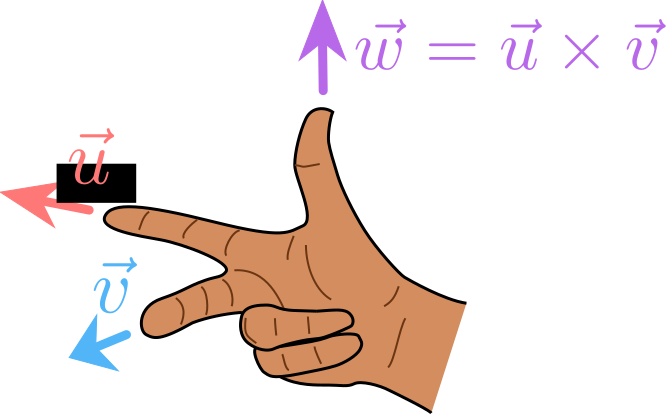
\includegraphics[scale=0.35]{cross_product/rhr.pdf}
  \end{figure}
\end{frame}

\begin{frame}
  \frametitle{The Cross Product}
  The cross product is \emph{anti-commutative}, i.e. changing the order of the vectors results in inverting the product:
  \begin{equation*}
  \rcolor{col1}{\vec{u}}\times\rcolor{col2}{\vec{v}} = -\left( \rcolor{col2}{\vec{v}}\times\rcolor{col1}{\vec{u}} \right).
  \end{equation*}

  \onslide<2>{
  When the vectors are given as column vectors $\rcolor{col1}{\vec{u}}=\colvec{3}{\rcolor{col1}{u_{x}}}{\rcolor{col1}{u_{y}}}{\rcolor{col1}{u_{z}}},\ \rcolor{col2}{\vec{v}}=\colvec{3}{\rcolor{col2}{v_{x}}}{\rcolor{col2}{v_{y}}}{\rcolor{col2}{v_{z}}}$, the resulting cross product is
  \begin{equation*}
  \rcolor{col1}{\vec{u}}\times\rcolor{col2}{\vec{v}} = \begin{pmatrix}\rcolor{col1}{u_{y}}\rcolor{col2}{v_{z}}-\rcolor{col1}{u_{z}}\rcolor{col2}{v_{y}}\\\rcolor{col1}{u_{z}}\rcolor{col2}{v_{x}}-\rcolor{col1}{u_{x}}\rcolor{col2}{v_{z}}\\\rcolor{col1}{u_{x}}\rcolor{col2}{v_{y}}-\rcolor{col1}{u_{y}}\rcolor{col2}{v_{x}}\end{pmatrix}
  \end{equation*}
  }
\end{frame}

\begin{frame}
  \frametitle{The Cross Product}
  \begin{presentation_example}
  What is the cross product of $\eb{1}=\colvec{3}{1}{0}{0}$ and $\eb{2}=\colvec{3}{0}{1}{0}$?
  \begin{equation*}
  \onslide<2->{
  \eb{1}\times\eb{2} = \begin{pmatrix}\cancel{0\cdot0}-\cancel{0\cdot1}\\\cancel{0\cdot0}-\cancel{1\cdot0}\\1\cdot1-\cancel{0\cdot0}\end{pmatrix}
  }
  \onslide<3->{
  = \colvec{3}{0}{0}{1}
  }
  \onslide<4->{
  = \eb{3}.
  }
  \end{equation*}
  \end{presentation_example}
\end{frame}

\begin{frame}
  \frametitle{The Cross Product}
  \begin{presentation_note}
  The cross product of two of the standard basis vectors in $\Rs{3}$ is the third basis vector. Its sign ($\pm$) is determined by a cyclic rule:
  \begin{equation*}
  \text{sign}\left( \eb{i}\times\eb{j} \right) =
  \begin{cases}
  1 & \text{if } (i,j)\in \left\{(1,2),\ (2,3),\ (3,1)\right\},\\
  -1 & \text{if } (i,j)\in \left\{(3,2),\ (2,1),\ (1,3)\right\},\\
  0 & \text{otherwise}.
  \end{cases}
  \end{equation*}
  \end{presentation_note}

  \onslide<2>{
  \begin{presentation_challenge}
  Using component calculation and utilizing the dot product, show that $\pcross{u}{v}$ is indeed orthogonal to both $\vec{u}$ and $\vec{v}$.
  \end{presentation_challenge}
  }
\end{frame}
